\documentclass[12pt]{book}

\usepackage[dvips,letterpaper,margin=0.75in,bottom=0.5in]{geometry}
\usepackage{cite}
\usepackage{slashed}
\usepackage{graphicx}
\usepackage{amsmath}
\usepackage{amssymb}
\usepackage{braket}
\begin{document}

\newcommand{\ihbar}{\ensuremath{i \hbar}}
\newcommand{\Pss}{\ensuremath{\Psi^*}}
\newcommand{\dPsidt}{\ensuremath{ \frac{\partial \Psi}{\partial t} }}
\newcommand{\dPsidx}{\ensuremath{ \frac{\partial \Psi}{\partial x} }}
\newcommand{\ddPsidx}{\ensuremath{ \frac{\partial^2 \Psi}{\partial x^2} }}
\newcommand{\dPssdt}{\ensuremath{ \frac{\partial \Psi^*}{\partial t} }}
\newcommand{\dPssdx}{\ensuremath{ \frac{\partial \Psi^*}{\partial x} }}
\newcommand{\ddPssdx}{\ensuremath{ \frac{\partial^2 \Psi^*}{\partial x^2} }}

\newcommand{\dphidt}{\ensuremath{ \frac{d \phi}{dt} }}
\newcommand{\dpsidx}{\ensuremath{ \frac{d \psi}{dx} }}
\newcommand{\ddpsidx}{\ensuremath{ \frac{d^2 \psi}{dx^2} }}


\title{PHY 115A \\ Lecture Notes 2B: \\ 
Tunneling and Scattering \\
(Griffith's 2.5-2.6,9.1-9.2)}
\author{Michael Mulhearn}

\maketitle

\setcounter{chapter}{1}
\chapter{Tunneling and Scattering}
\setcounter{section}{25}
\setcounter{equation}{70}

\section{Continuity of the Wave Function}

Let's consider with the case $V(x)$ is finite everywhere, then we start from the TISE:
$$-\frac{\hbar^2}{2m}\,\frac{d^2 \psi}{d x^2} + V(x) \, \psi(x) = E \, \psi(x)$$
Without loss of generality, we'll investigate continuity at $x=0$, by integrating the TISE from $-\epsilon$ to $+\epsilon$:
$$\int_{-\epsilon}^{+\epsilon}\frac{d^2 \psi}{d x^2} dx = \frac{2m}{\hbar^2}\int_{-\epsilon}^{+\epsilon} \left(V(x) - E\right) \; \psi(x) \, dx$$
We'll assume that we keep $\epsilon > 0$ here and everywhere below.  By the fundamental theorem of calculus the LHS is:
\begin{equation}
\label{eqn:psicont}
\left. \frac{d\psi}{d x} \right\rvert_{+\epsilon} 
- \left. \frac{d\psi}{d x} \right\rvert_{-\epsilon}
 = \frac{2m}{\hbar^2}\int_{-\epsilon}^{+\epsilon} \left(V(x) - E\right) \; \psi(x) \, dx
\end{equation}
In the limit $\epsilon \to 0$, the RHS vanishes since $V(x)$ is finite, so:
$$ \lim_{\epsilon \to 0} \left( \left. \frac{d\psi}{d x} \right\rvert_{+\epsilon} 
- \left. \frac{d\psi}{d x} \right\rvert_{-\epsilon} \right) = 0$$
which is to say the derivative of the wave function is continuous, and so the wave function is continuous as well.

But what about infinite (or undefined) $V(x)$?  Here we still insist that the wave function be continuous, as otherwise the state of a particle would be undefined at some point.  But the derivative need not be continuous, as the $V(x)$ term in LHS in Equation~\ref{eqn:psicont} no longer vanishes in the limit $\epsilon \to 0$:
\begin{equation}
\label{eqn:psidiscont}
\lim_{\epsilon \to 0} \left( \left. \frac{d\psi}{d x} \right\rvert_{+\epsilon} 
- \left. \frac{d\psi}{d x} \right\rvert_{-\epsilon} \right) = 
\lim_{\epsilon \to 0}
\frac{2m}{\hbar^2}\int_{-\epsilon}^{+\epsilon} V(x) \; \psi(x) \, dx
\end{equation}

\section{The Dirac Delta Function}

The so-called ``Dirac Delta Function'' $\delta(x)$ is defined by it's behavior in an integral:
\begin{equation}
\int_{-\infty}^{+\infty} f(x) \, \delta(x) \, dx = f(0) 
\end{equation}
where it ``picks out'' the value of $f(x)$ at $x=0$.  It immediately follows (put $f(x)=1$) that:
\begin{equation}
\int_{-\infty}^{+\infty} \delta(x) \, dx = 1 
\end{equation}
Also, changing variables to make the subsitutions clearer:
$$\int_{-\infty}^{+\infty} g(y) \, \delta(y) \, dy = g(0)$$
and putting $y = x - a$, we get:
$$\int_{-\infty}^{+\infty} g(x-a) \, \delta(x-a) \, dy = g(0)$$
and defining $f(x) \equiv g(x-a)$ we have:
\begin{equation}
\int_{-\infty}^{+\infty} f(x) \, \delta(x-a) \, dy = f(a)
\end{equation}
The Dirac Delta Function isn't really a function at all, but it is often described as one:
$$\delta(x) = \begin{cases}
0, & x \neq 0 \\
\infty, & x=0 \\
\end{cases}
$$
but such a definition shouldn't be taken too seriously.  A better way is to consider it is as a limit of perfectly reasonable functions with integral one, that get narrower and narrower around 0.  Just as the limit of a series of rational numbers can be an irrational number, the $\delta$-function is the limit of a sequence of square-integrable functions, but isn't itself square integrable.  We could try:
\begin{equation*}
\int_{-\infty}^{+\infty} \delta^2(x) \, dy = \delta(0)
\end{equation*}
but what are we to make of $\delta(0)$? At best, we could say it is in infinity.  Mathematician's call the $\delta$-function a generalized function or distribution.  It only makes sense in the context of its defining integral equation above, and doesn't exist as a function on its own.  If you think of what we actually do with wave functions (calculate integrals) this isn't really any limitation at all.

For $x \neq 0$, $\delta(x) = 0$ is well defined.  But otherwise, just stick to its well defined properties (the numbered equations here) within integrals, and we will see the $\delta$-function is extremely useful.

\section{Bound State of the Delta Function Potential}

We turn to the very useful example a delta function potential.
\begin{equation}
V(x) = -\alpha \delta(x) 
\end{equation}
Since we've agreed to never discuss the delta function at $x=0$ outside of an integral, we will just say that $V(x)$ does not have a defined minimum, and so we are free to see if there are normalizable solution with $E<0$.  

Away from $x=0$, where $\delta(x)$ is well defined, $V(x)=0$ and the TISE is:
\begin{equation*}
\frac{d^2 \psi}{d x^2} = -\frac{2mE}{\hbar^2}\psi(x) = \kappa^2 \psi(x), \hspace{2cm} \kappa \equiv \frac{\sqrt{-2mE}}{\hbar}.
\end{equation*}
which has general solutions:
$$\psi(x) = A e^{\displaystyle - \kappa x} + B e^{\displaystyle \kappa x}$$
But for the wave function to be well defined only:
$$\psi(x) = A e^{\displaystyle - \kappa x}, \hspace{2cm} x>0$$ 
and
$$\psi(x) = B e^{\displaystyle \kappa x}, \hspace{2cm} x<0$$
are acceptable.  From continuity of the wave function at $x=0$, we conclude:
$$A=B$$
and write $\psi(x)$ as:
$$\psi(x) = \begin{cases}
B e^{\displaystyle \kappa x} &  x\leq0 \\
B e^{\displaystyle -\kappa x} &  x\geq0 \\
\end{cases}
$$
We saw above that the presence of the $\delta$-function means the wave function need not be continuous at $x=0$, and in fact:
\begin{eqnarray*}
\lim_{\epsilon \to 0} \left( \left. \frac{d\psi}{d x} \right\rvert_{+\epsilon} 
- \left. \frac{d\psi}{d x} \right\rvert_{-\epsilon} \right) &=& 
\lim_{\epsilon \to 0}
\frac{2m}{\hbar^2}\int_{-\epsilon}^{+\epsilon} V(x) \, \Psi(x) \, dx \\
&=& 
\lim_{\epsilon \to 0}
\frac{2m}{\hbar^2}\int_{-\epsilon}^{+\epsilon} \left( -\alpha \delta(x) \right) \Psi(x)\, dx\\
&=& \lim_{\epsilon \to 0} \left( -\frac{2m\alpha}{\hbar^2} \psi(0) \right) \\
&=& -\frac{2m\alpha}{\hbar^2} \psi(0) \\ 
\end{eqnarray*}
In our case:
$$\psi(0) = B$$
and:
$$\frac{d\psi}{dx} = \begin{cases}
\kappa B e^{\displaystyle \kappa x} &  x\leq0 \\
-\kappa B e^{\displaystyle -\kappa x} &  x\geq0 \\
\end{cases}
$$
so:
$$
\lim_{\epsilon \to 0} \left( \left. \frac{d\psi}{d x} \right\rvert_{+\epsilon} 
- \left. \frac{d\psi}{d x} \right\rvert_{-\epsilon} \right) = -\kappa B - \kappa B = 
-\frac{2m\alpha}{\hbar^2} B 
$$
or
$$\kappa = \frac{m\alpha}{\hbar^2}$$
or
$$E = -\frac{\hbar^2 \kappa^2}{2m} = - \frac{m\alpha^2}{2\hbar^2}$$
Normalizing the wave function is left as an exercise, it yields:
$$|B|^2 = \kappa$$

Now, consider the case where $V(x)=+\alpha \delta(x)$ If we stubbornly
refuse to define the minimum of the wave function in the presence of a
delta function (even though in this case it is going to positive
infinity, so we are being very careful here!) we should check if there
are solutions for $E<0$.  But notice in this case that the boundary
conditions on the derivative would lead to $\kappa < 0$, and so now
the exponential terms blow up at $+\infty$ and $-\infty$ instead of
going to zero.

\section{Scattering States of the Delta Function Well}

For the case that $E>0$, we have the free particle TISE for $x<0$:
\begin{equation*}
\frac{d^2 \psi}{d x^2} = -\frac{2mE}{\hbar^2}\psi(x) = -k^2 \psi(x), \hspace{2cm} k \equiv \frac{\sqrt{2mE}}{\hbar}.
\end{equation*}
with general solution:
$$\psi(x) = A e^{\displaystyle ikx} + B e^{\displaystyle -ikx}$$
Similarly, for $x>0$ the general solution is:
$$\psi(x) = F e^{\displaystyle ikx} + G e^{\displaystyle -ikx}$$
and so:
$$\psi(x) = \begin{cases}
A e^{\displaystyle ikx} + B e^{\displaystyle -ikx} &  x\leq0 \\
F e^{\displaystyle ikx} + G e^{\displaystyle -ikx} &  x\geq0 \\
\end{cases}
$$
and:
$$\frac{d\psi}{dx} = \begin{cases}
(iAk) e^{\displaystyle ikx} + (-iBk) e^{\displaystyle -ikx} &  x\leq0 \\
(iFk) e^{\displaystyle ikx} + (-iGk) e^{\displaystyle -ikx} &  x\geq0 \\
\end{cases}
$$
Continuity of $\psi(x)$ at $x=0$ requires:
$$F+G=A+B$$
and from:
$$
\lim_{\epsilon \to 0} \left( \left. \frac{d\psi}{d x} \right\rvert_{+\epsilon} 
- \left. \frac{d\psi}{d x} \right\rvert_{-\epsilon} \right) = 
-\frac{2m\alpha}{\hbar^2} \psi(0) 
$$
so:
\begin{eqnarray*}
ik(F-G-A+B) &=& -\frac{2m\alpha}{\hbar^2} (A+B) \\
F-G &=& (A-B)+i\frac{2m\alpha}{k\hbar^2} (A+B) \\
\end{eqnarray*}
Finally:
$$F-G = A (1+2i\beta) - B (1-2i\beta) $$
where:
$$\beta = \frac{m \alpha}{\hbar^2 k}$$
For scattering from the left, let $A$ represent the (known) incident wave and set
$$G=0$$ so that now we have two equations and two unknowns:
$$F = A + B$$
and:
$$F = A (1+2i\beta) - B (1-2i\beta) $$
Solving for $F$ in terms of $A$:
\begin{eqnarray*}
F &=& A (1+2i\beta) - (F-A)\,(1-2i\beta)\\
2F(1-i\beta) &=& 2A 
\end{eqnarray*}
and so:
$$F = \frac{A}{1-i\beta}$$
similarlyy:
$$B = \frac{i\beta}{1-i\beta}$$
The reflection coefficient is:
$$R = \frac{|B|^2}{|A|^2} = \frac{\beta^2}{1+\beta^2}$$
and:
$$T = \frac{|F|^2}{|A|^2} = \frac{1}{1+\beta^2}$$
Notice that:
$$R+T=1$$
Now let's look at what happens for:
$$V(x) = +\alpha \delta(x)$$
Nothing changes until we reach the boundary condition on the derivative, which becomes:
$$
\lim_{\epsilon \to 0} \left( \left. \frac{d\psi}{d x} \right\rvert_{+\epsilon} 
- \left. \frac{d\psi}{d x} \right\rvert_{-\epsilon} \right) = 
+\frac{2m\alpha}{\hbar^2} \psi(0) 
$$
So we can read off the solutions for this case by putting $\beta \to -\beta$ in the solutions above, which leaves the transmission and reflection unchanged.


\section{Bound States of the Finite Square Well}

Next we consider the finite square well potential:
$$V(x) = \begin{cases}
-V_0, & -a \leq x \leq a \\
0     & {\rm otherwise} \\
\end{cases}
$$
As the potential is finite everywhere, we expect both $\psi$ and $d\psi/dx$ to be continuous.
The bound state potentials will have $-V_0 < E < 0$.  For $x < -a$ and $x > a$, we encounter a familiar form of the TISE:
\begin{equation*}
\frac{d^2 \psi}{d x^2} = -\frac{2mE}{\hbar^2}\psi(x) = \kappa^2 \psi(x), \hspace{2cm} \kappa \equiv \frac{\sqrt{-2mE}}{\hbar}.
\end{equation*}
with the solutions
$$\psi(x) = A e^{\displaystyle \kappa x}$$
for $x<-a$ and
$$\psi(x) = B e^{\displaystyle -\kappa x}$$
for $x>a$.  Within the potential well at $-a \leq x \leq a$ we have:
\begin{equation*}
\frac{d^2 \psi}{d x^2} = -\frac{2m(V_0+E)}{\hbar^2}\psi(x) = -k^2 \psi(x), \hspace{2cm} k \equiv \frac{\sqrt{2m(V_0 + E)}}{\hbar}.
\end{equation*}
with general solution:
$$\psi(x) = C \sin(kx) + D \cos(kx)$$
At this point, we will save ourselves a lot of hassle by noting that $V(x)$ is even, and so the general solutions can be constructed as either even or odd solutions\footnote{See Griffith's P2.1c.  Or note that if $\psi(x)$ is a solution, so is $\psi(-x)$, and we can add or subtract the two to get even and odd solutions.}  So we need only establish continuity for $x \geq 0$ and we will automatically have it for $x \leq 0$.

Starting with the even solutions and $x\geq0$, we write:
$$\psi(x) = \begin{cases}
Be^{\displaystyle -\kappa x} & x > a \\
D \cos(kx) & 0 \leq x \leq a \\
\end{cases}$$
and continuity implies:
\begin{equation}
\label{eqn:fswcont}
B e^{-\kappa a} = D \cos(ka)
\end{equation}
We see that the dimensionless quantities $\kappa a$ and $ka$ are of interest, so it will simplify things to note that:
$$(ka)^2+(\kappa a)^2 = \frac{-2mEa^2}{\hbar^2} + \frac{2m(E+V_0)a^2}{\hbar^2} = 
\frac{2mV_0a^2}{\hbar^2} \equiv z_0^2$$
The derivative is:
$$\frac{d\psi}{dx} = \begin{cases}
-\kappa \, B \, e^{\displaystyle -\kappa x} & x > a \\
-kD \sin(kx) & 0 \leq x \leq a \\
\end{cases}$$
which both must be continuous at $x=a$, so:
\begin{eqnarray*}
-\kappa B e^{-\kappa a} &=& -k D \sin(ka)\\
 \kappa B e^{-\kappa a} &=& k D \sin(ka)\\
 (\kappa a) B e^{-\kappa a} &=& (ka) D \sin(ka)\\
\end{eqnarray*}
where we have multiplied by $a$ so that the equation is in terms of the dimensionless constants $ka$ and $\kappa a$.  Dividing by Equation~\ref{eqn:fswcont} we obtain:
\begin{eqnarray*}
\kappa a &=& (ka) \, \tan(ka) \\
\sqrt{z_0^2-(ka)^2} &=& (ka) \, \tan(ka) \\
\sqrt{z_0^2-z^2} &=& z \, \tan(z) \\
\end{eqnarray*}
where we have defined 
$$z \equiv ka = \frac{\sqrt{2m(E+V_0)}a}{\hbar}$$
and so finally:
\begin{equation}
\sqrt{\left(\frac{z_0}{z}\right)^2-1} = \tan(z) 
\end{equation}
This is an equation with no known algebraic solution.  It can be solved graphically or numerically.  See Fig.~\ref{fig:finitewell}.
\begin{figure}[thb]
\begin{center}
{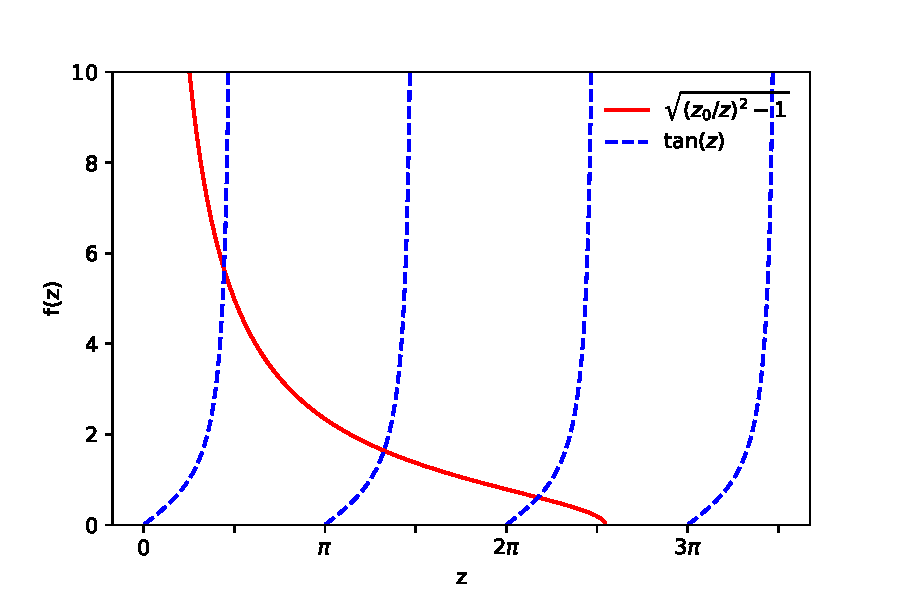
\includegraphics[width=0.60\textwidth]{python/finitewell.pdf}}
\end{center}
\caption{\label{fig:finitewell} The allowed energies for the finite potential occur at the intersection of these curves.}
\end{figure}
There are some interesting limiting cases to consider.  When:
$$z_0 < \frac{\pi}{2}$$
there is only one bound state (we haven't found the odd solutions yet, which is why this is $\pi/2$ and not $\pi$, as you might expect from the figure...)  Recalling the definition for $z_0$, this amounts to:
$$V_0\,a^2 < \frac{\pi^2 \hbar^2}{8m}$$
which defines a shallow and narrow well.

Alternative, if $z_0$ is very large, then the intersection points are at:
$$z = \frac{n\pi}{2}, \hspace{2cm} n=1,3,5,\ldots$$
which means the allowed energies are:
$$E + V_0 = \frac{n^2\pi^2\hbar^2}{2m(2a)^2}$$
which (relative to the bottom of the well) are the energies of the infinite square well.

\section{Scattering States of the Finite Square Well}

For $E>0$, we have only free particle solutions, but with two different wave numbers, so we'll take:
$$k \equiv \frac{\sqrt{2mE}}{\hbar^2}, \hspace{1cm }{\rm and} \hspace{1cm} k' \equiv \frac{\sqrt{2m(E+V_0)}}{\hbar^2}$$
with:
$$\frac{k'}{k} = \sqrt{\frac{E+V_0}{E}} \equiv \eta$$
and so:
$$k' = \eta k$$
Note that if this was an optics problem we would call $\eta$ the refractive index.  The piecewise general solution to the TISE is:
\begin{eqnarray*}
\psi(x) = \begin{cases}
A e^{\displaystyle ikx} + B e^{\displaystyle -ikx} & x < -a \\ 
C e^{\displaystyle i\eta kx} + D e^{\displaystyle -i\eta kx} & -a \leq x \leq a \\ 
F e^{\displaystyle ikx} + G e^{\displaystyle -ikx} & x > a \\ 
\end{cases}
\end{eqnarray*}
but we are going to write it this way instead:
\begin{eqnarray*}
\psi(x) = \begin{cases}
A e^{\displaystyle ik(x+a)} + B e^{\displaystyle -ik(x+a)} & x < -a \\ 
C e^{\displaystyle i\eta kx} + D e^{\displaystyle -i\eta kx} & -a \leq x \leq a \\ 
F e^{\displaystyle ik(x-a)} + G e^{\displaystyle -ik(x-a)} & x > a \\ 
\end{cases}
\end{eqnarray*}
which will make it much easier to evaluate at the boundaries ($x=\pm a$).  We are free to do this because:
$$A e^{ik(x+a)} = (A e^{ika}) e^{ikx}$$
where $A$ is a constant we have not yet determined.  The derivative is:
\begin{eqnarray*}
\frac{d\psi}{dx} = \begin{cases}
ik \left(Ae^{\displaystyle ik(x+a)} - B e^{\displaystyle -ik(x+a)}\right) & x < -a \\ 
i\eta k \left(Ce^{\displaystyle i\eta kx} - D e^{\displaystyle -i \eta k x}\right) & -a \leq x \leq a \\ 
ik \left(Fe^{\displaystyle ik(x-a)} - G e^{\displaystyle -ik(x-a)}\right) & x > a \\ 
\end{cases}
\end{eqnarray*}

Define:
$$\alpha \equiv e^{i\eta ka}$$
and note that:
$$|\alpha|^2 = 1$$
which will be useful later.  Now the four continuity equations are:
\begin{eqnarray*}
A + B &=& C \alpha^* + D \alpha \\
A - B &=& \eta(C \alpha^* - D \alpha) \\
C \alpha + D \alpha^* &=& F + G  \\
\eta(C \alpha - D \alpha^*) &=& F - G \\
\end{eqnarray*}
The incoming waves are $A$ and $G$.  In principle, we can use two equations to eliminate the intermediate waves $C$ and $D$.  Then we can use the remaining two to calculate the outgoing waves $B$ and $F$ from the incoming waves $A$ and $G$. 

Note that the first two equations can be added to eliminate $B$:
$$A = \frac{(\eta+1) \alpha^*}{2} \, C - \frac{(\eta-1) \alpha}{2} \, D$$
But now let's make our lives a little easier and set $G=0$.  Then the last two equations become:
\begin{eqnarray*}
\alpha C  + \alpha^* D &=& F   \\
\eta \alpha C  - \eta \alpha^* D &=& F  \\
\end{eqnarray*}
Which we use to solve for $C$ and $D$ in terms of $F$:
$$C = \frac{\eta+1}{2\eta}\alpha^* F$$
and:
$$D = \frac{\eta-1}{2\eta}\alpha F$$
Plugging these back in to our expression for $A$:
\begin{eqnarray*}
A &=& \frac{(\eta+1)^2 (\alpha^2)^* - (\eta-1)^2 \alpha^2}{4 \eta} \, F \\
  &=& \frac{\eta^2+1}{2\eta}\,\frac{(\alpha^2)^*-\alpha^2}{2}+\frac{(\alpha^2)^*+\alpha^2}{2}\\
\end{eqnarray*}
Recalling our definition for $\alpha$:
$$A/F = \cos(2\eta ka) - i\frac{\eta^2+1}{2\eta} \sin(2\eta ka)$$
and so the transmission is:
\begin{eqnarray*}
\frac{1}{T} = \frac{|A|^2}{|F|^2} &=& \cos^2(2\eta ka) + \frac{(\eta^2+1)^2}{4\eta^2} \sin^2(2\eta ka) \\
&=& 1 + \left(\frac{(\eta^2+1)^2}{4\eta^2} - 1\right)\sin^2(2\eta ka) \\
&=& 1 + \frac{\eta^2-1}{4\eta^2}\sin^2(2\eta ka)\\
\end{eqnarray*}
Notice that the transmission is one when either:
$$\eta=1$$
which corresponds to know change in index of refraction, i.e. $V_0=0$.  Or:
$$\sin^2(2\eta ka) $$
that is when:
$$ 2a\frac{\sqrt{2m(E+V_0)}}{\hbar}= n \pi$$
or:
$$E+V_0 = \frac{n^2 \pi^2 \hbar^2}{2m (2a)^2}$$
which you may recognize at the allowed energies from the infinite potential well.


\section{The WKB Approximation and the ``Classical'' Region}

The inspiration for this approximation comes from the free particle, with wave function:
$$\psi(x) = A \exp(\pm ikx)$$
Consider a particle in a region where the potential $V$ is constant, and $E>V$.  Then the wave function is the same as the free particle but with:
$$k=\sqrt{2m(E-V)}/\hbar$$
We are going to try to extend this solution to the case that the potential is slowly varying.  By slowly, we mean that $\psi(x)$ oscillates many times before the potential changes significantly.  In this case, we anticipate that $\psi(x)$ will continue to oscillate, but the amplitude and phase will change slowly.  We will therefore look for solutions of the form:
\begin{equation}
\Psi(x) = A(x) \, e^{\displaystyle i \phi(x)}
\end{equation}
where:
$$A(x) \in \mathbb{R}, \hspace{1cm} {\rm and} \hspace{1cm} \phi(X) \in \mathbb{R}$$
Our approximation is that $A(x)$ is slowly varying, in the sense that:
$$\left| \frac{1}{A} \, \frac{d^2A}{dx^2}\right| << \left| \frac{1}{\psi}\,\frac{d^2 \psi}{dx^2} \right|$$
In a region where $E > V(x)$ we can write the SE as:
\begin{equation}
\label{eqn:wkbse}
\frac{d^2 \psi}{d x^2} = -\frac{p^2(x)}{\hbar^2} \psi(x)
\end{equation}
where
$$p(x) = \sqrt{2m(E-V(x))}$$
And so we can write our approximation as:
$$\left| \frac{A''}{A} \right| << \left| \frac{\psi''}{\psi} \right| = \frac{p^2(x)}{\hbar^2}$$

Returning to:
$$\psi(x) = A(x) \, e^{\displaystyle i \phi(x)}$$
we have:
$$\frac{d\psi}{d x} = \left(A' + i\,A\,\phi'\right)\; e^{\displaystyle i \phi(x)}$$
and:
\begin{eqnarray*}
\frac{d^2 \psi}{d x^2} &=&  \left\{A'' + i\,A'\,\phi' + i\,A\,\phi''
+ \left(A' + i\,A\,\phi'\right)\; i \phi' \right\} \; e^{\displaystyle i \phi(x)} \\
&=& \left\{\left(A''-A\left(\phi'\right)^2\right) + i\left(2\,A'\,\phi' + A\,\phi''\right)\right\}\; e^{\displaystyle i \phi(x)} \\
-\frac{p^2}{\hbar^2}\,A&=& 
\left(A''-A\left(\phi'\right)^2\right) + i\left(2\,A'\,\phi' + A\,\phi''\right)\\
\end{eqnarray*}
where in the last line we have used Equation~\ref{eqn:wkbse}.  Since $A$ and $\phi$ are real, this amounts to two equations (one for the real and one for the imaginary part):
\begin{equation}
\label{eqn:wkbfirst}
-\frac{p^2}{\hbar^2}\,A = \left(A''-A\left(\phi'\right)^2\right)
\end{equation}
and
\begin{equation}
\label{eqn:wkbsecond}
2A'\phi'+A\phi'' = 0
\end{equation}
We first solve Equation~\ref{eqn:wkbsecond} by noting:
$$\left(A^2\phi'\right)' = \left(2AA'\phi'+A^2\phi''\right) = A \left(2A'\phi'+A\phi''\right) = 0$$
So:
$$A^2 \phi' = C^2$$
and:
$$A(x) = \frac{C}{\sqrt{\phi'}}$$
so we need only find $\phi(x)$ and we will have $A(x)$.  That should come from solving Equation~\ref{eqn:wkbsecond} which we write as:
$$\left(\phi'\right)^2 = \frac{p^2}{\hbar^2} + \frac{A''}{A}$$
We cannot solve this in general, but we have already decided to make the approximation that $A(x)$ is varying slowly:
$$\left| \frac{A''}{A} \right| \ll \frac{p^2}{\hbar^2} $$
This approximation leads to:
\begin{eqnarray*}
\left(\phi'\right)^2 &=& \frac{p^2}{\hbar^2}\\
\frac{d\phi}{dx} &=& \pm \, \frac{p}{\hbar}\\
\end{eqnarray*}
and so:
$$A(x) = \frac{C}{\sqrt{\phi'}} = \frac{C\sqrt{\hbar}}{\sqrt{p(x)}}$$
Integrating $\phi'$ we get:
$$\phi(x) = \pm \frac{i}{\hbar} \left( \int p(x) dx + D\right)$$
where $D$ is a constant of integration.  Assembling this all together we get:
$$\psi(x) = \frac{C \, \sqrt{\hbar} \, e^{\pm iD/\hbar}}{\sqrt{p(x)}} \exp\left(\pm\frac{i}{\hbar}\int p(x) \, dx \right)$$
which we can write as:
\begin{equation}
\psi(x) = \frac{C}{\sqrt{p(x)}} \exp\left(\pm\frac{i}{\hbar}\int p(x) \, dx \right)
\end{equation}
where $C$ here is a new complex constant.  Notice that:
$$|\psi(x)|^2 = \frac{|C|^2}{p(x)}$$


\section{Bound states of an Infinite Square Well with a Bumpy Bottom}

Consider the example of the an infinite square well with some function $f(x)$ along the bottom (instead of $V(x)=0$) for $0 < x < a$.  The WKB approximation gives us the general solution:

$$\psi(x)=\frac{1}{\sqrt{p(x)}}\left(C\,e^{\displaystyle i\phi(x)} 
+ D\,e^{\displaystyle -i\phi(x)}\right)$$

where we calculate:
$$\phi(x) = \frac{1}{h}\int_0^x p(x) dx$$
Notice that we are free to choose the starting point for integration, and we need only take the postive version, since we've included $\pm\phi(x)$ in the general solution. 
Since $\phi(0)=0$, and we must have $\psi(0)=0$, then we have:
$$C+D=0 \implies D = -C$$
and so:
$$\psi(x) = \frac{C}{\sqrt{p(x)}}\,\left(e^{\displaystyle i\phi(x)} 
+ D\,e^{\displaystyle -i\phi(x)}\right)
= \frac{i\,2\,C}{\sqrt{p(x)}}\sin(\phi(x)
$$
which we can write as:
$$\psi(x) = \frac{C}{\sqrt{p(x)}}\sin(\phi(x))$$
by absorbing other factors into the constant $C$.  Now we must also have:
$$\psi(x)=0$$
which we requires that:
$$\phi(x) = n\pi$$
or:
$$\int_0^a p(x) dx = n\pi \hbar$$
Notice that for $V(x)=0$ we have $p(x) = \sqrt{2mE}$ and so:
$$\int_0^a p(x) dx = \sqrt{2mE}a = n \pi \hbar$$
or:
$$E_n = \frac{n^2 \pi^2 \hbar^2}{2\,m\,a^2}$$

\end{document}




